\begin{figure}[htbp]
    \centering
    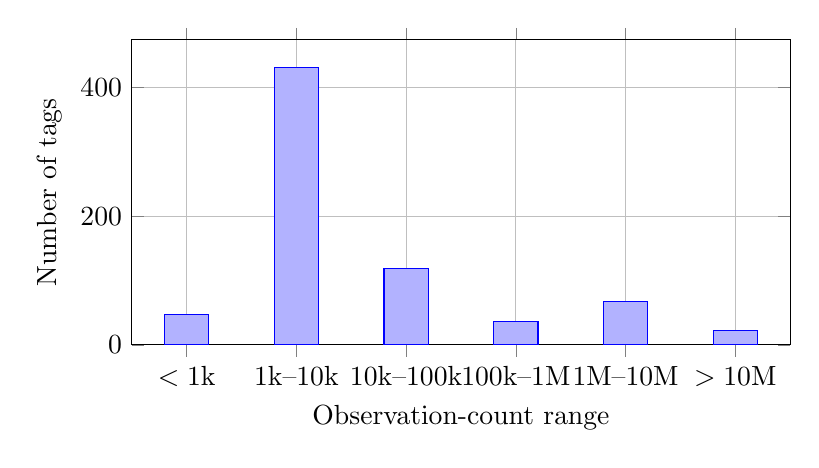
\begin{tikzpicture}
    \begin{axis}[
        width=0.82\linewidth,
        height=0.45\linewidth,
        ybar,
        bar width=16pt,
        xlabel={Observation-count range},
        ylabel={Number of tags},
        xtick={1,2,3,4,5,6},
        xticklabels={{$<1$k},{1k--10k},{10k--100k},{100k--1M},{1M--10M},{$>10$M}},
        ymin=0,
        grid=major
    ]
        \addplot coordinates {
(1,47)
(2,431)
(3,118)
(4,37)
(5,68)
(6,22)
        };
    \end{axis}
    \end{tikzpicture}
    \caption{Distribution of sensor tags by observation-count magnitude in the lift-aligned raw dataset.}
    \label{fig:tag-count-magnitude}
\end{figure}
